% =============================================================================
% The CGAL Developers' Manual
% Chapter: Polymorphic Return Types
% -----------------------------------------------------------------------------
% file   : objects.tex
% authors: Stefan Schirra <stschirr@mpi-sb.mpg.de>
% -----------------------------------------------------------------------------
% $Revision$
% $Date$
% =============================================================================

\chapter{Polymorphic Return Types}
\ccChapterAuthor{Stefan Schirra ({\tt stschirr@mpi-sb.mpg.de})}
\ccIndexMainItem{polymorphism}%
\ccIndexMainItem{polymorphic return types}
For some geometric operations, the type of the result of the operation
is not fixed a priori, but depends on the input. Intersection computation
is a prime example. The standard object-oriented approach to this is defining
a common base class for all possible result types and returning a reference 
or a pointer to an object of the result type by a reference or pointer to the
base class. Then all the virtual member functions in the interface of 
the base class can be applied to the result object and the implementation
corresponding to the actual result type is called. It is hard to define
approriate base class interface functions (besides \ccc{draw()}).

\cgal\ has chosen a different approach, since \cgal\ wants to avoid large
class hierarchies. With the \cgal\ 
class \ccc{Object}\ccIndexMainItem[C]{Object}, you can fake a common
base class\ccIndexSubitem{base class}{faking}, see Figure \ref{Fig:Object}. 

\begin{figure}[h]
\lcTex{
\begin{center}
  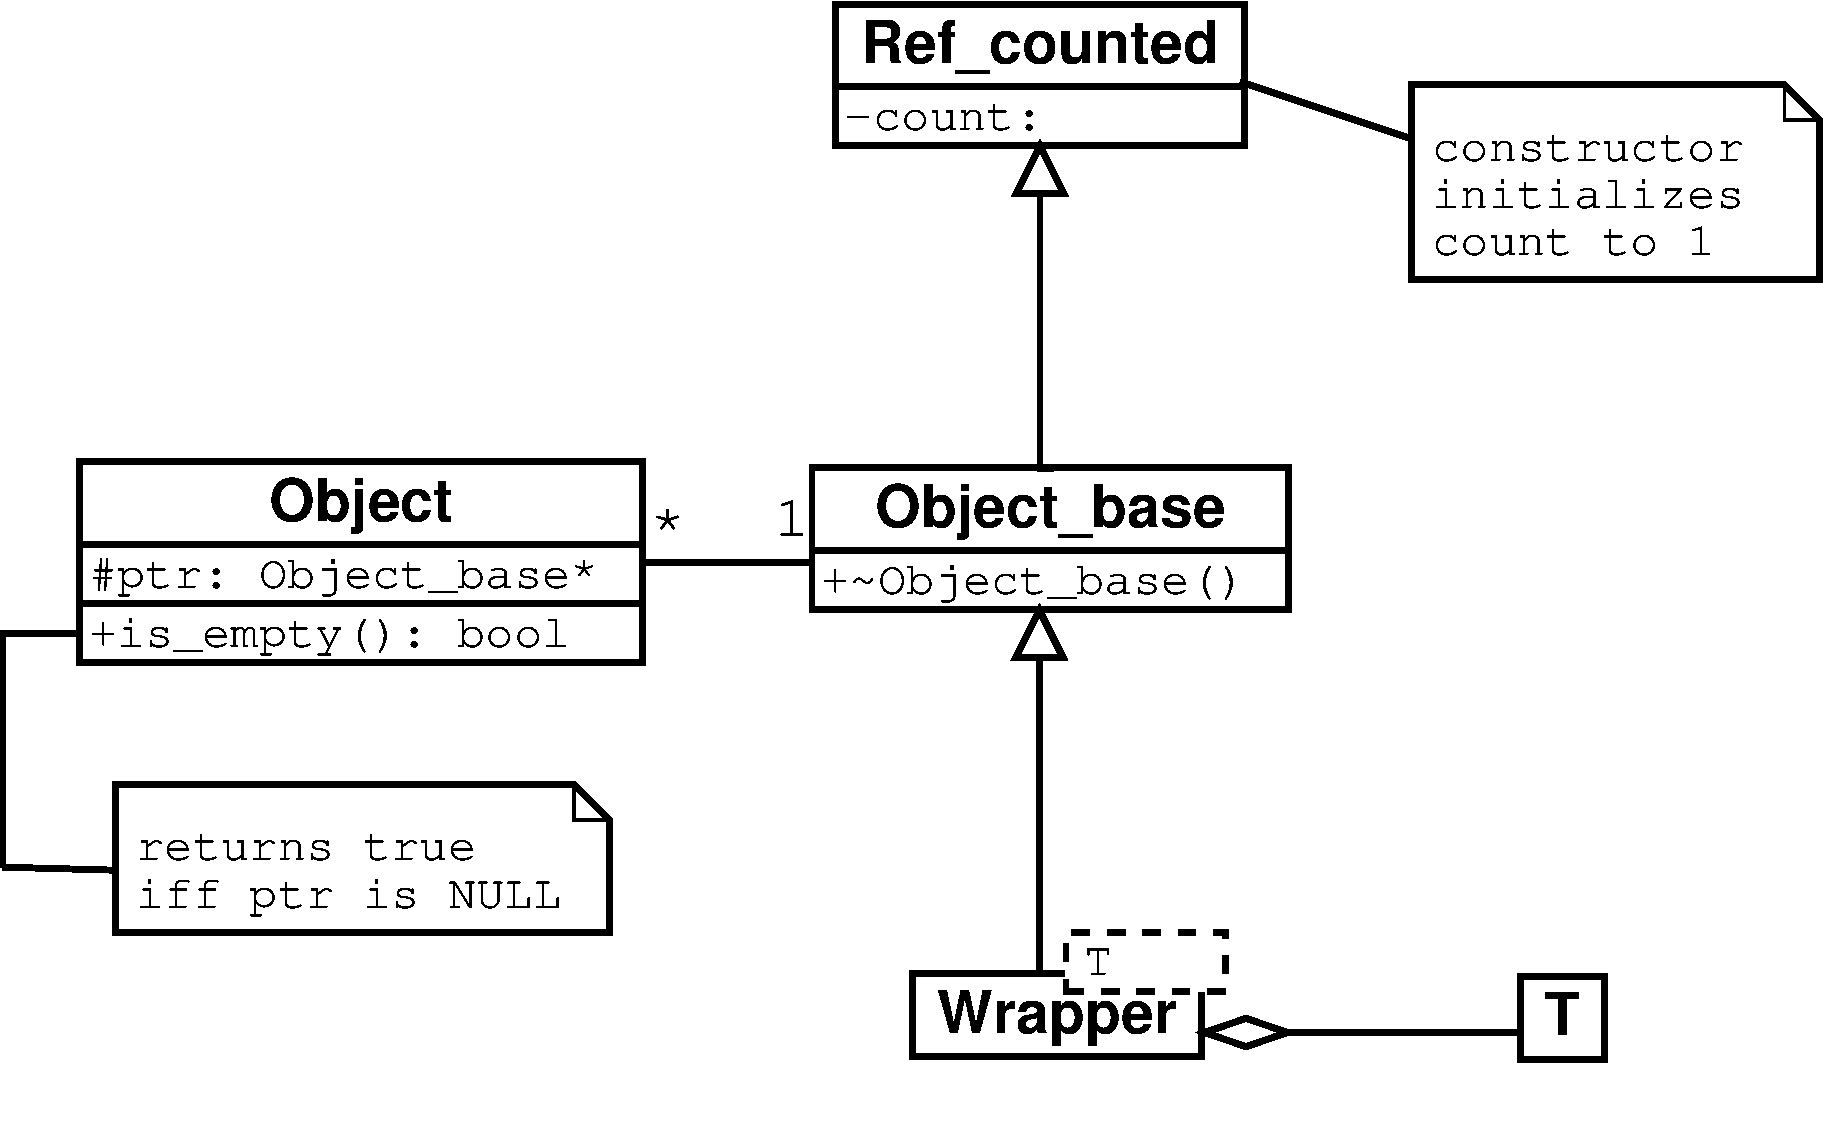
\includegraphics[width=11cm]{Developers_manual/fig/Object}
\end{center}
}
\caption{UML class diagram for faked object hierarchies (since 2.2-I-4).\label{Fig:Object}}
\lcRawHtml{
<CENTER>
<IMG BORDER=0 SRC="fig/Object.gif"
   ALT="Faked object heirarchies UML diagram"><BR>
</CENTER>
}
\end{figure}

Functions having a polymorphic return type create an object of the actual
result type and wrap it into an object of type \ccc{Object}.
You can use the \ccc{make_object()}\ccIndexGlobalFunction{make_object}
function to do this. 
\begin{verbatim}
template <class R>
Object
intersection(const Plane_3<R>& plane1, const Plane_3<R>& plane2);
\end{verbatim}
The following piece of code is taken from the above \cgal\ intersection routine:
\begin{verbatim}
    if (det != zero) 
    {
        is_pt = Point_3<R>(zero, c*s-d*r, d*q-b*s, det);
        is_dir = Direction_3<R>(det, c*p-a*r, a*q-b*p);
        return make_object(Line_3<R>(is_pt, is_dir));
    }
\end{verbatim}

There is only one member operation defined for \ccc{Object}, a test for
an empty object. In order to make use of the returned object, 
you can try to assign it to the possible return types using 
\ccc{CGAL::assign(Candidate_return_type, Object)}\ccIndexGlobalFunction{assign}
function; see also the definition of the class 
\ccAnchor{http://www.cgal.org/Manual/doc_html/kernel/Class_Object.html}{\ccc{Object}} in the 
\cgal\ kernel manual. 

For functions potentially computing more than one polymorphic objects, some 
\cgal\ functions use \ccc{std::list<CGAL::Object>} as return value. 
\begin{verbatim}
std::list<CGAL::Object>
fct_might_return_several_objects_of_different_types(...);
\end{verbatim}

A more generic approach is the use of \ccc{OutputIterators}, just like
the \stl\ does:
\begin{verbatim}
template <typename OutputIterator>
OutputIterator
fct_might_return_several_objects_of_different_types(..., OutputIterator result);
\end{verbatim}
where \ccc{iterator_traits<OutputIterator>::value_type} must be \ccc{Object}.
The sequence of objects returned starts with the output iterator passed to
the function. The output iterator returned is the past-the-end iterator of 
the constructed sequence of objects. 

